\newpage
\subsection{Caso d'uso UC5: Recupero password }
\label{UC5}
\begin{figure}[ht]
	\centering
	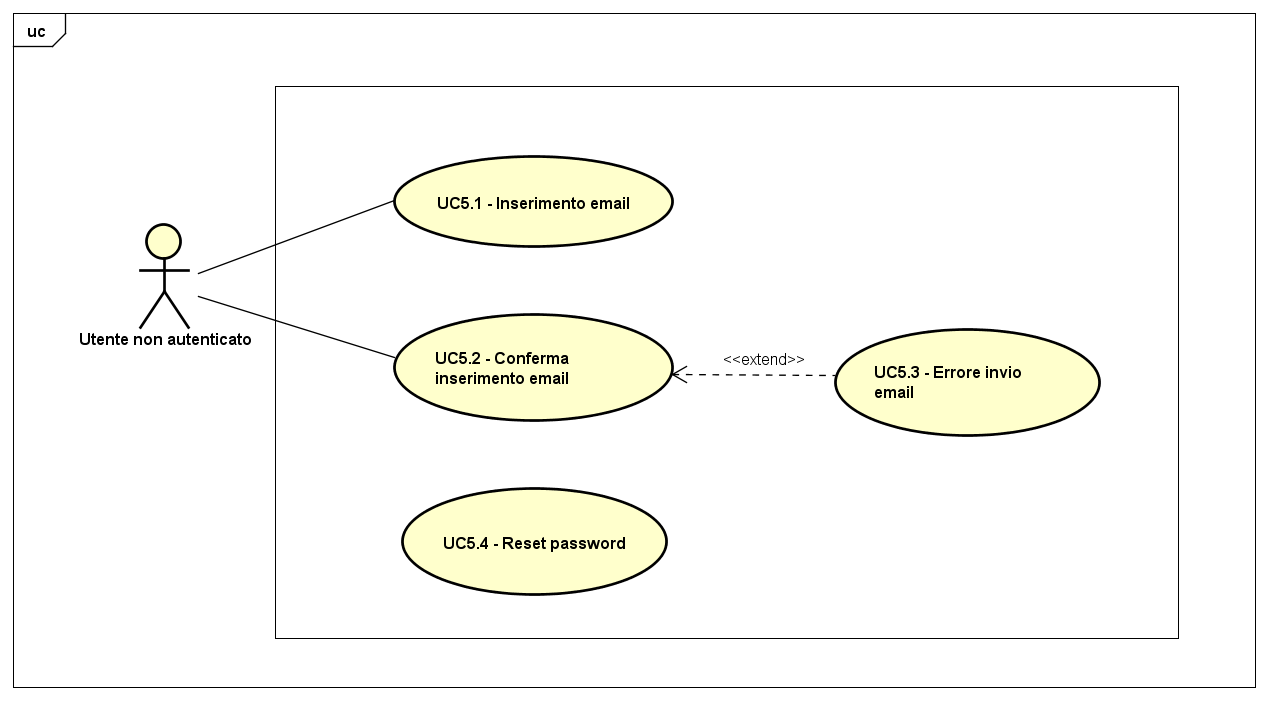
\includegraphics[scale=0.45]{UML/UC5.png}
	\caption{UC5: Recupero password }
\end{figure}

\begin{longtable}{ l | p{11cm}}
	\hline
	\rowcolor{Gray}
	 \multicolumn{2}{c}{UC5 - Recupero password} \\
	 \hline
	\textbf{Attori} & Utente non autenticato \\
	\textbf{Descrizione} & L'attore tenta il recupero della propria password tramite l'invio di una email \\
	\textbf{Pre-Condizioni} & L'attore ha scelto di recuperare la sua password e non è autenticato \\
	\textbf{Post-Condizioni} & L'attore ha ricevuto nella propria casella email un link per reimpostare la propria password, oppure la procedura è fallita \\
	\textbf{Scenario Principale} & 
	\begin{enumerate*}[label=(\arabic*.),itemjoin={\newline}]
		\item L'attore può inserire la propria email di registrazione (UC5.1)
		\item L'attore può confermare l'indirizzo email inserito, al quale l'applicazione web ha inviato un link per reimpostare la password (UC5.2)
	\end{enumerate*}\\
	\textbf{Scenari Alternativi} & 
	\begin{enumerate*}[label=(\arabic*.),itemjoin={\newline}]
		\item L'attore visualizza un errore e l'invio della email di recupero password non avviene (UC5.3) 
	\end{enumerate*}\\
\end{longtable}